\begin{frame}
  \frametitle{Interaction implies heterogeneity}
  The interaction index measures the contribution of the interaction terms:

  \begin{itemize}
    \item \(f(x_1, x_2) = x_1^2 + \log(x_2) + \alpha x_1x_2^3\)
    \item \(\alpha = 0.1 \rightarrow\) low interaction index \(\rightarrow\) high fidelity
    \item \(\alpha = 100 \rightarrow\) high interaction index \(\rightarrow\) low fidelity
    \end{itemize}
  \noindent\makebox[\linewidth]{\rule{\paperwidth}{0.4pt}}
  But it does not say how the interaction terms influence the feature effect plots
\end{frame}


\begin{frame}
  \frametitle{Example}
  \begin{figure}
    \centering
    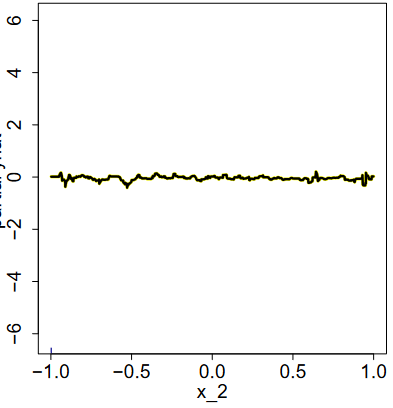
\includegraphics[width=0.5\textwidth]{pdp}
    \caption{PDP plot, taken from \href{https://arxiv.org/abs/1309.6392}{Goldstein et. al}}
  \end{figure}
  \noindent\makebox[\linewidth]{\rule{\paperwidth}{0.4pt}}
  Interpretation?
  Maybe $y \perp\!\!\!\!\perp x_2$
\end{frame}

\begin{frame}
  \frametitle{Example}
  \begin{figure}
    \centering
    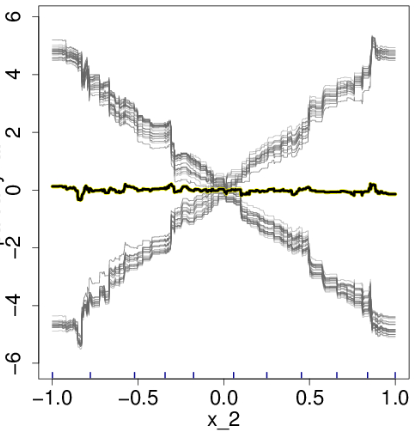
\includegraphics[width=0.5\textwidth]{pdp_ice}
    \caption{PDP-ICE plot, taken from \href{https://arxiv.org/abs/1309.6392}{Goldstein et. al}}
  \end{figure}
  \noindent\makebox[\linewidth]{\rule{\paperwidth}{0.4pt}}
  Interpretation now? Maybe $y \approx \pm 6 x_2 $ depending on a condition
\end{frame}

\begin{frame}
  \frametitle{Heterogeneity on PDP is called ICE}
  \begin{itemize}
    \item Local effects, often, deviate from the global effect
    \item Aggregation bias $\rightarrow$ \href{https://arxiv.org/pdf/1908.09635.pdf}{Mehrabi et. al. (2019)}
    \item $\mathtt{ICE}^{(i)}(x_s) = f(x_s, \mathbf{x}_c^{(i)})$
    \item Another approach $\rightarrow \mathbb{V}(x_s) = \frac{1}{N-1}\sum_i \left ( f(x_s, x_c^{(i)}) - \underbrace{\frac{1}{N} \sum_i f(x_s, x_c^{(i)})}_{\mu(x_s)} \right)^2$
    \item ICE show the \emph{type} of heteronegeneity, variance shows only the \emph{magnitude}
    \item They both model the uncertainty of the feature effect!
  \end{itemize}
  \noindent\makebox[\linewidth]{\rule{\paperwidth}{0.4pt}}
  ICE have the same limitations as PDPs under correlations!
\end{frame}

\begin{frame}
  \frametitle{Heterogeneity/Uncertainty on ALE}
  \begin{itemize}
    \item The variance idea?
    \item Estimate the variance inside each bin?
    \item And then aggregate the variances?
    \item Bin splitting is important, otherwise biased estimation of the variance
  \end{itemize}
  \noindent\makebox[\linewidth]{\rule{\paperwidth}{0.4pt}}
  Spoiler; we are working on it!
\end{frame}


\begin{frame}
  \frametitle{Regional Effect plots}
  \begin{itemize}
    \item Heterogeneity $\rightarrow$ subspaces with homogeneous effects
  \end{itemize}

  \begin{figure}
    \centering
    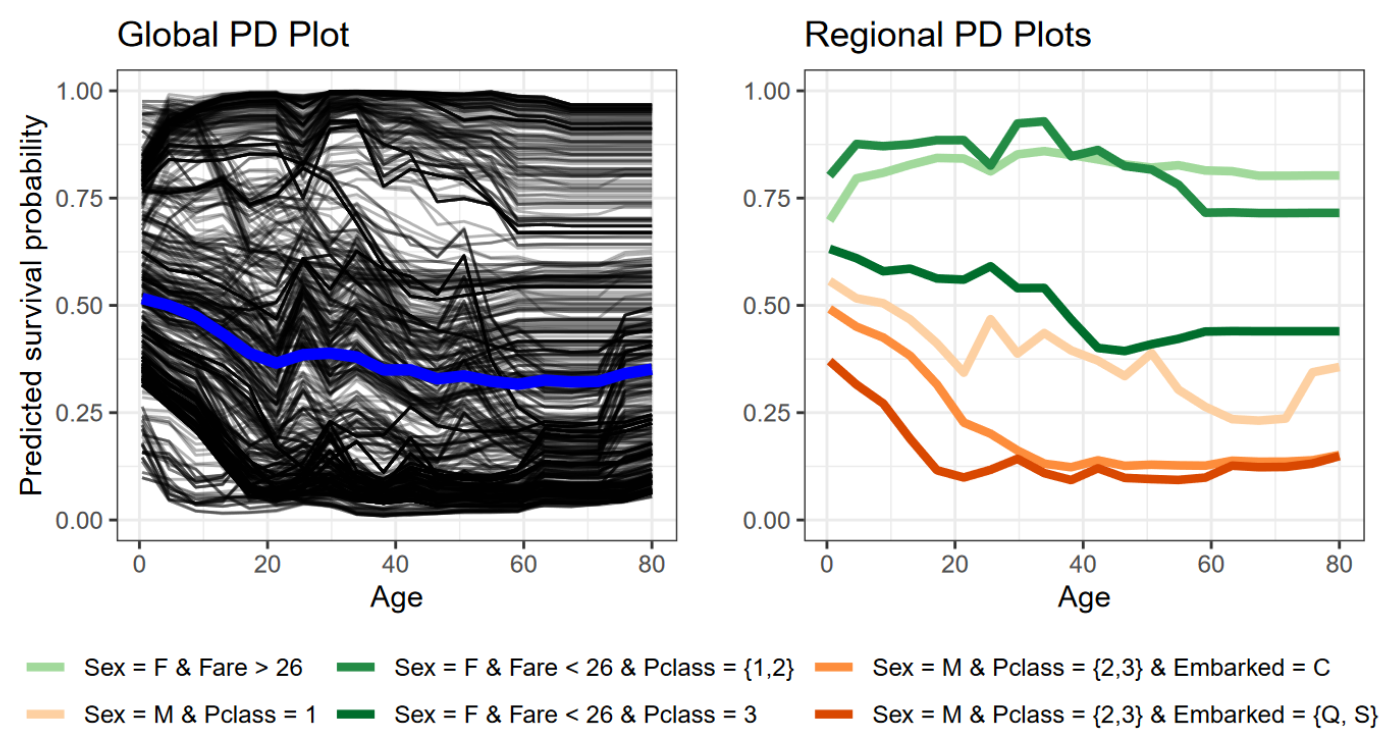
\includegraphics[width=0.9\textwidth]{repid}
    \caption{REPID: Regional Effect plots, taken from \href{https://arxiv.org/abs/2202.07254}{Herbinger et. al}}
  \end{figure}
\end{frame}

